%%
%% This is file `tikzposter-template.tex',
%% generated with the docstrip utility.
%%
%% The original source files were:
%%
%% tikzposter.dtx  (with options: `tikzposter-template.tex')
%% 
%% This is a generated file.
%% 
%% Copyright (C) 2014 by Pascal Richter, Elena Botoeva, Richard Barnard, and Dirk Surmann
%% 
%% This file may be distributed and/or modified under the
%% conditions of the LaTeX Project Public License, either
%% version 2.0 of this license or (at your option) any later
%% version. The latest version of this license is in:
%% 
%% http://www.latex-project.org/lppl.txt
%% 
%% and version 2.0 or later is part of all distributions of
%% LaTeX version 2013/12/01 or later.
%% 






\documentclass[17pt, a1paper, landscape, margin=0mm, innermargin=15mm,
blockverticalspace=15mm, colspace=15mm, subcolspace=8mm]{tikzposter}
% \documentclass{tikzposter} %Options for format can be included here
% \setcolumnnumber{3}
 % Title, Author, Institute
\title{\textbf{Mysterious Meerkat}, QA System, CS6340, Fall 2015}
\author{\textbf{Debjyoti Paul}, deb@cs.utah.edu }
\institute{\textbf{School of Computing, University of Utah}}
\titlegraphic{

\includegraphics[width=0.14\textwidth]{figures/ulogo.png}
}

%%%%%%%%% Awesome tex stack exchange answer 
% http://tex.stackexchange.com/questions/167521/tikz-poster-aligning-titlegraphic-to-the-right-of-the-title
%%%%%%%%%%%%%%%%%%%%%%%%%%%%%%%%%%%%%%%%%%%%%%%%%%%

\makeatletter
\renewcommand\TP@maketitle{%
   \centering
         \tikz[remember picture,overlay]\node[scale=0.8,anchor=east,xshift=0.5\linewidth,yshift=2.3cm,inner sep=0pt] {%
       \@titlegraphic
    };
   \begin{minipage}[b]{0.8\linewidth}
        \centering
        \color{titlefgcolor}
        {\bfseries \Huge \sc \@title \par}
        \vspace*{1em}
        {\huge \@author \par}
        \vspace*{1em}
        {\LARGE \@institute}
    \end{minipage}%
}
\makeatother


%Choose Layout
\usetheme{Basic}
% \usecolorpalette{PurpleGrayBlue}
\usecolorstyle{qacolor}
\usebackgroundstyle{BottomVerticalGradation}

\usetitlestyle{Envelope}

\begin{document}

 % Title block with title, author, logo, etc.
\maketitle
\begin{columns}
\column{0.33}
 \block{QA SYSTEM STRUCTURE}{
 \begin{tikzfigure}[Basic Question Answering System ]
\label{fig:fig1}
\includegraphics[width=0.25\textwidth]{figures/basic.png}
\end{tikzfigure}
 }
\note[targetoffsetx=3.2cm, targetoffsety=-10cm, angle=20, rotate=12]
{
Since \textbf{Reading Comprehension Test} has defined domain of search space, our QA system does not require \textbf{Document Retrieval module}. Our focus is mainly in building an efficient \textbf{Answer Processing} module.
}
 
\column{0.33}
 \block{INTRODUCTION}{
  Human beings have an inherent tendency to seek information. In the world of internet useful information is free flowing. However we are more interested in getting specific answer to queries rather than just gathering relevant information.
  \\[10pt]
  \textbf{Question Answering (QA) system} is a specialized form of Information Retrieval. QA is in itself intersection of \textbf{Natural Language Processing, Information Retrieval, Information Extraction, Machine Learning, Knowledge Representation, Logic and Inference, Sematic Search}.  \textbf{QA Systems} are needed everywhere, be it medical science, learning systems for students, personal assistants. 
  \\[10pt]
  Here in this project we are more concerned in answering quesions for Reading Comprehension tests where domain of search is defined. 
 }
\column{0.33}
 \block{AFTERTHOUGHTS}{
\begin{itemize}
\\[-0.5in]
\item[] \textbf{Things went well}
    \begin{enumerate}
    \item Question classifier to determine answer type as HUM:ind, HUM:gr, LOC:city, NUM:date, NUM:money is the key to enhance performance.
    \item Using regex to find number, date and currency such as 'dd[??] [Month]' in date, 1800-2100 for Years and \$100.0 or \$ 0.50 for currency has helped.
    \item The idea of measure of the length of the shortest path in the semantic ontology between two words. Also extracting verb from question and finding matching verbs  or its synset has improved system performance
    \end{enumerate}
\end{itemize}
\begin{itemize}
\item[] \textbf{Things could have been better}
    \begin{enumerate}
    \item Coreference resolution has little effect on my QA system, might need to revamp scoring function to see its effect.
    \end{enumerate}
\end{itemize}

 }
\end{columns}
 \begin{columns}
 % FIRST column
\column{0.2}% Width set relative to text width
\block{MODULES}{
\begin{itemize}
\item[] \textbf{Question Processing Module}
    \begin{enumerate}
    \item Question Classifier
    \item Answer Type Detector
    \end{enumerate}
\item[] \textbf{Answer Processing Module}
    \begin{enumerate}
    \item Named Entity Extractor
            \begin{itemize}
            \item Human 
            \item Location
            \end{itemize}
    \item Sentence Similarity module
            \begin{itemize}
            \item \emph{Verb and theme Extractor}
            \item \emph{Synset and Hypernym matching module}
            \end{itemize}
    \item Answer type rule based module
            \begin{itemize}
            \item \emph{Human Individual / Group}
            \item \emph{Number Count / Money / Date / Period / Size / Weight etc.}
            \item \emph{Location country / city / other}
            \item \emph{Reasoning answer}
            \end{itemize}
    \end{enumerate}
\item[] \textbf{Answer Formulation Module}
    \begin{enumerate}
    \item Number, Name, Location extractor
    \end{enumerate}
\end{itemize}
}

\note[targetoffsetx=9.2cm, targetoffsety=-6.5cm, angle=-90, width=0.35\textwidth, rotate=1]
{
\emph{Did you know?} \\
In 2000 Semantic and Rule based QA system gained much attention; Researchers around the globe gathered and contributed to form a QA research roadmap; Our instructor \textbf{E. Riloff} has also made contribution in it.
}

 % SECOND column
\column{0.5}
 %Second column with first block's top edge aligned with with previous column's top.
\block{}{
 \begin{tikzfigure}[ Inside Answering Module ]
\label{fig:fig2}
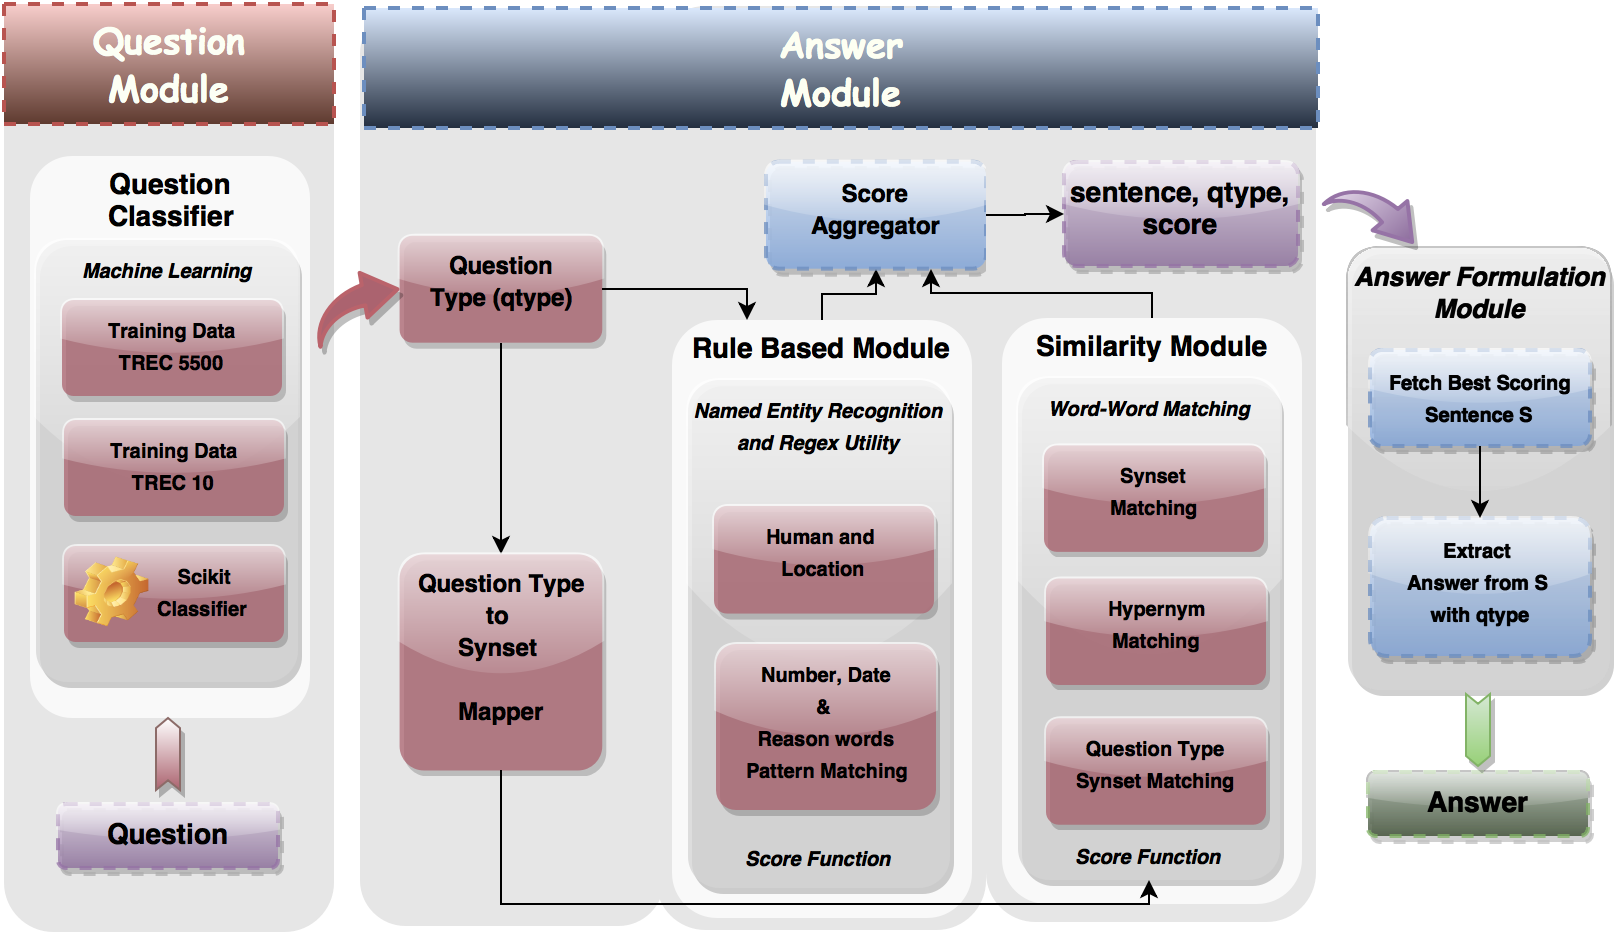
\includegraphics[width=0.45\textwidth]{figures/answer.png}
\end{tikzfigure}
 }

\note[targetoffsetx=-0.2cm, targetoffsety=15cm, angle=-10, width=0.3\textwidth, rotate=-4]
{\emph{Note:}\\
  \textbf{Preprocessing module} is not shown in diagram. In preprocessing step the passage is passed through an \textbf{Anaphora Resolution system}(i.e. \textbf{BART-Beautiful Anaphore resolution Toolkit)} ) to resolute pronomial coreferences; with a hypothesis that it will help answering module to find answer.
}

\column{0.3}

\block[titleleft]{CITATIONS}{
\begin{enumerate}
\item Question Classifiers is based on the Paper \textbf{Learning Question Classifiers: The Role of Semantic Information}, Xin Li, Dan Roth, \emph{Natural Language Engineering}, 2004
\item Some concept of Sentence Similarity Module is borrowed from  Paper \textbf{Sentence Similarity Based on Semantic Nets and Corpus Statistics} by Yuhua Li, David McLean et. al.
\item Coreference Module: \textbf{BART Beautiful Anaphora Resolution Tool} by Massimo Poesio et.al.
\item Ofcourse worth to mention our NLP friend \textbf{NLTK} and \textbf{Scipy} 
\end{enumerate}
}
\note[targetoffsetx=-1.2cm, targetoffsety=4.2cm, angle=30, width=0.115\textwidth, rotate=4]
{\emph{Did you know?}\\ First \textbf{Neural Network} based Factoid QA on passage was published last year, 2014, by M. Iyyer of UMD.
}

\note[targetoffsetx=-8.2cm, targetoffsety=-2.2cm, angle=-95, width=0.10\textwidth, rotate=-10]
{
\emph{Did you know?}\\ \textbf{SIRI} was primarily a QA project started in \textbf{2003} funded by \textbf{DARPA} till 2008 and everyone came to know about it after being integrated with apple \textbf{iOS4} in 2010.
}

\block[titleright, bodywidthscale=.8, bodyinnersep=-4em]{ $f(x)$ SCORING }{
\begin{minipage}[t]{1in}
\end{minipage}
\hfill
\begin{minipage}[t]{5in}
 1. Rule Based scores \textbf{ $0 \leq f_1(x) \leq 1 $} \\
 2. \textbf{0.25} for best matching, \textbf{0.15} for probable \\ \hspace*{0.15in} \textbf{0.05} for may be answers.\\
 3. Scoring function of Similarity Module \\ 
 \hspace*{0.15in} \textbf{$0 \leq f_2(x) \leq 1 $} \\
\end{minipage}
\hspace*{1in} 
4. Hypernyms matched words score is less than the synsets matched words $f_2(hypernym) < f_2(synset)$ \\

\centerline{\textsc{ScoreAggregator} = $ f_1(x) * (1+f_2(x)) $} \hfill
}

%%%%%%%%% Suggestion from 
% http://tex.stackexchange.com/questions/233854/tikz-poster-block-title-colours
%%%%%%%%%%
{
\colorlet{notebgcolor}{colorOne!10!white}

}
%  \block{QA SYSTEM HISTORY}{
%  \textbf{[1968-71]} Terry Winograd, MIT Artificial Intelligence Laboratory developed \textbf{SHRDLU} where computer can answer short block of response to query.\\
%  \textbf{[1978]}  Lehnert\'s thesis, first to proposed a question answering system based on semantics and reasoning.\\
%  \textbf{[1980s]} \textbf{LUNAR} and \textbf{BASEBALL} QA system appears\\
%  \textbf{[1993]} START by Boris Katz, first web based QA system at CSAIL, MIT\\
%  \textbf{[2000]} \textbf{Semantic and rule based QA system} gained attention, QA Roadmap paper published. Contirbution from well known researchers around the globe; including E. Riloff. (Our cs6340 Instructor)\\
%  \textbf{[2003]} \textbf{SIRI} started in 2003 funded by DARPA till 2008. Integrated with apple iOS4 in 2010.\\
%  \textbf{[2007-2011]} \textbf{IBM Watson},  it was a breakthrough in open domain
% Question Answering System.
%  }

\end{columns}

\end{document}



\endinput
%%
%% End of file `tikzposter-template.tex'.
